% ════════════════════════════════════════════
% 运用方法概述（02.总体分析.tex）
% ════════════════════════════════════════════
\section{运用方法概述}
\subsection{分析框架}

本报告的分析对象是同一品牌主页的 500 条帖子，核心任务是识别曝光量的影响因素，并把回归系数翻译为可执行的投放建议。分析按“数据诊断—数据整理—回归建模—效应测算”四个环节递进：数据诊断判断数据能支持什么样的模型，数据整理把原始数据整理为可回归的分析数据，回归建模估计并诊断模型，效应测算把模型结果转换为曝光增量、倍数与置信区间。四个环节共享同一份只读原始数据与同一套变量口径，前一环节的输出直接作为后一环节的输入。

\subsection{方法组合}

数据诊断环节以描述统计、相关分析与方差分解为主。描述统计给出曝光量的均值、分位数、偏度与峰度，判断是否需要变换；Pearson 与 Spearman 相关分别刻画线性与单调同步程度；以月份哑变量对粉丝规模对数做辅助回归，并把总方差拆为月间与月内两部分，用解释度与月内方差占比判断两个变量是否属于同一变异维度。判别标准取相关系数绝对值不低于 0.9、辅助回归解释度不低于 0.9、月内方差占比低于 5\%，三项同时满足即视为不可同时识别。

数据整理环节以规则核查与变量变换为主。缺失按列统计并用众数填补二元变量，重复按全部原始字段比对，越界只标记不修改；名义变量做独热编码并指定参照类，周期性的时段按凌晨、上午、下午晚间合并，连续变量取对数、计数型因变量取 log1p。为检验处理方案的影响，另以删除缺失行的样本重估同一模型，比较核心系数的差异。

回归建模环节以多元线性回归为骨架，配合 HC3 异方差稳健标准误。共线用方差膨胀因子、广义方差膨胀因子与标准化设计矩阵条件数三角度诊断；模型设定按“全模型—剔除粉丝规模—剔除月份—仅线性月份—最终模型”递进比较；残差用 Jarque--Bera、Breusch--Pagan、White、Ramsey RESET 与 Cook 距离检验；预测能力用十折交叉验证评估；变量组的解释贡献用 Shapley 分解量化。

效应测算环节以 Duan 烟雾还原与反事实模拟为主。先在对数尺度预测，再用残差经验分布构造的烟雾因子还原到曝光次数；在代表性画像与全样本两个层面构造付费与自然、视频与图片的反事实；用 1000 次多元正态参数模拟传播系数不确定性；对内容主题做联合 Wald 检验与两两检验；最后在六种模型设定下复核效应方向与量级，并按内容主题分组检验付费效应的异质性。

\subsection{技术路线}

整个流程围绕一条主线展开：先由共线判别决定粉丝规模与月份谁进入模型，再在编码后的数据上估计、筛选并诊断模型，最后把系数还原为曝光尺度并给出区间。具体而言，以 $\log(1+Y_i)$ 为因变量、以发帖决策变量与月份固定效应为解释变量估计回归；用 $R^2$、调整 $R^2$、整体 $F$ 与十折交叉验证比较 M0 至 M4；用 VIF、条件数与增量 $F$ 判断共线来源；用 JB、BP、White、RESET 与 Cook 距离检查残差；用 Shapley 分解回答“曝光方差中有多少可归因于发帖决策”；用烟雾还原与参数模拟把系数翻译为曝光次数与倍数。后文的数值与图表都沿这条主线产生，可以在同一份分析数据上复现。

图\ref{fig:route}把上述流程按四个任务分组呈现：任务 1 数据理解确定变量类型、粒度与结构，输出变量字典与因果角色；任务 2 清洗与编码给出缺失填补、哑变量构造与 $\log(1+Y_i)$ 变换；任务 3 以 OLS 加 HC3 稳健标准误估计模型，并以 VIF、残差检验与十折交叉验证诊断；任务 4 把系数还原为付费提升百分比、视频相对图片的倍数，并在六种设定下复核稳健性。四个任务串行推进，前一任务的输出即后一任务的输入。

\begin{figure}[htbp]
  \centering
  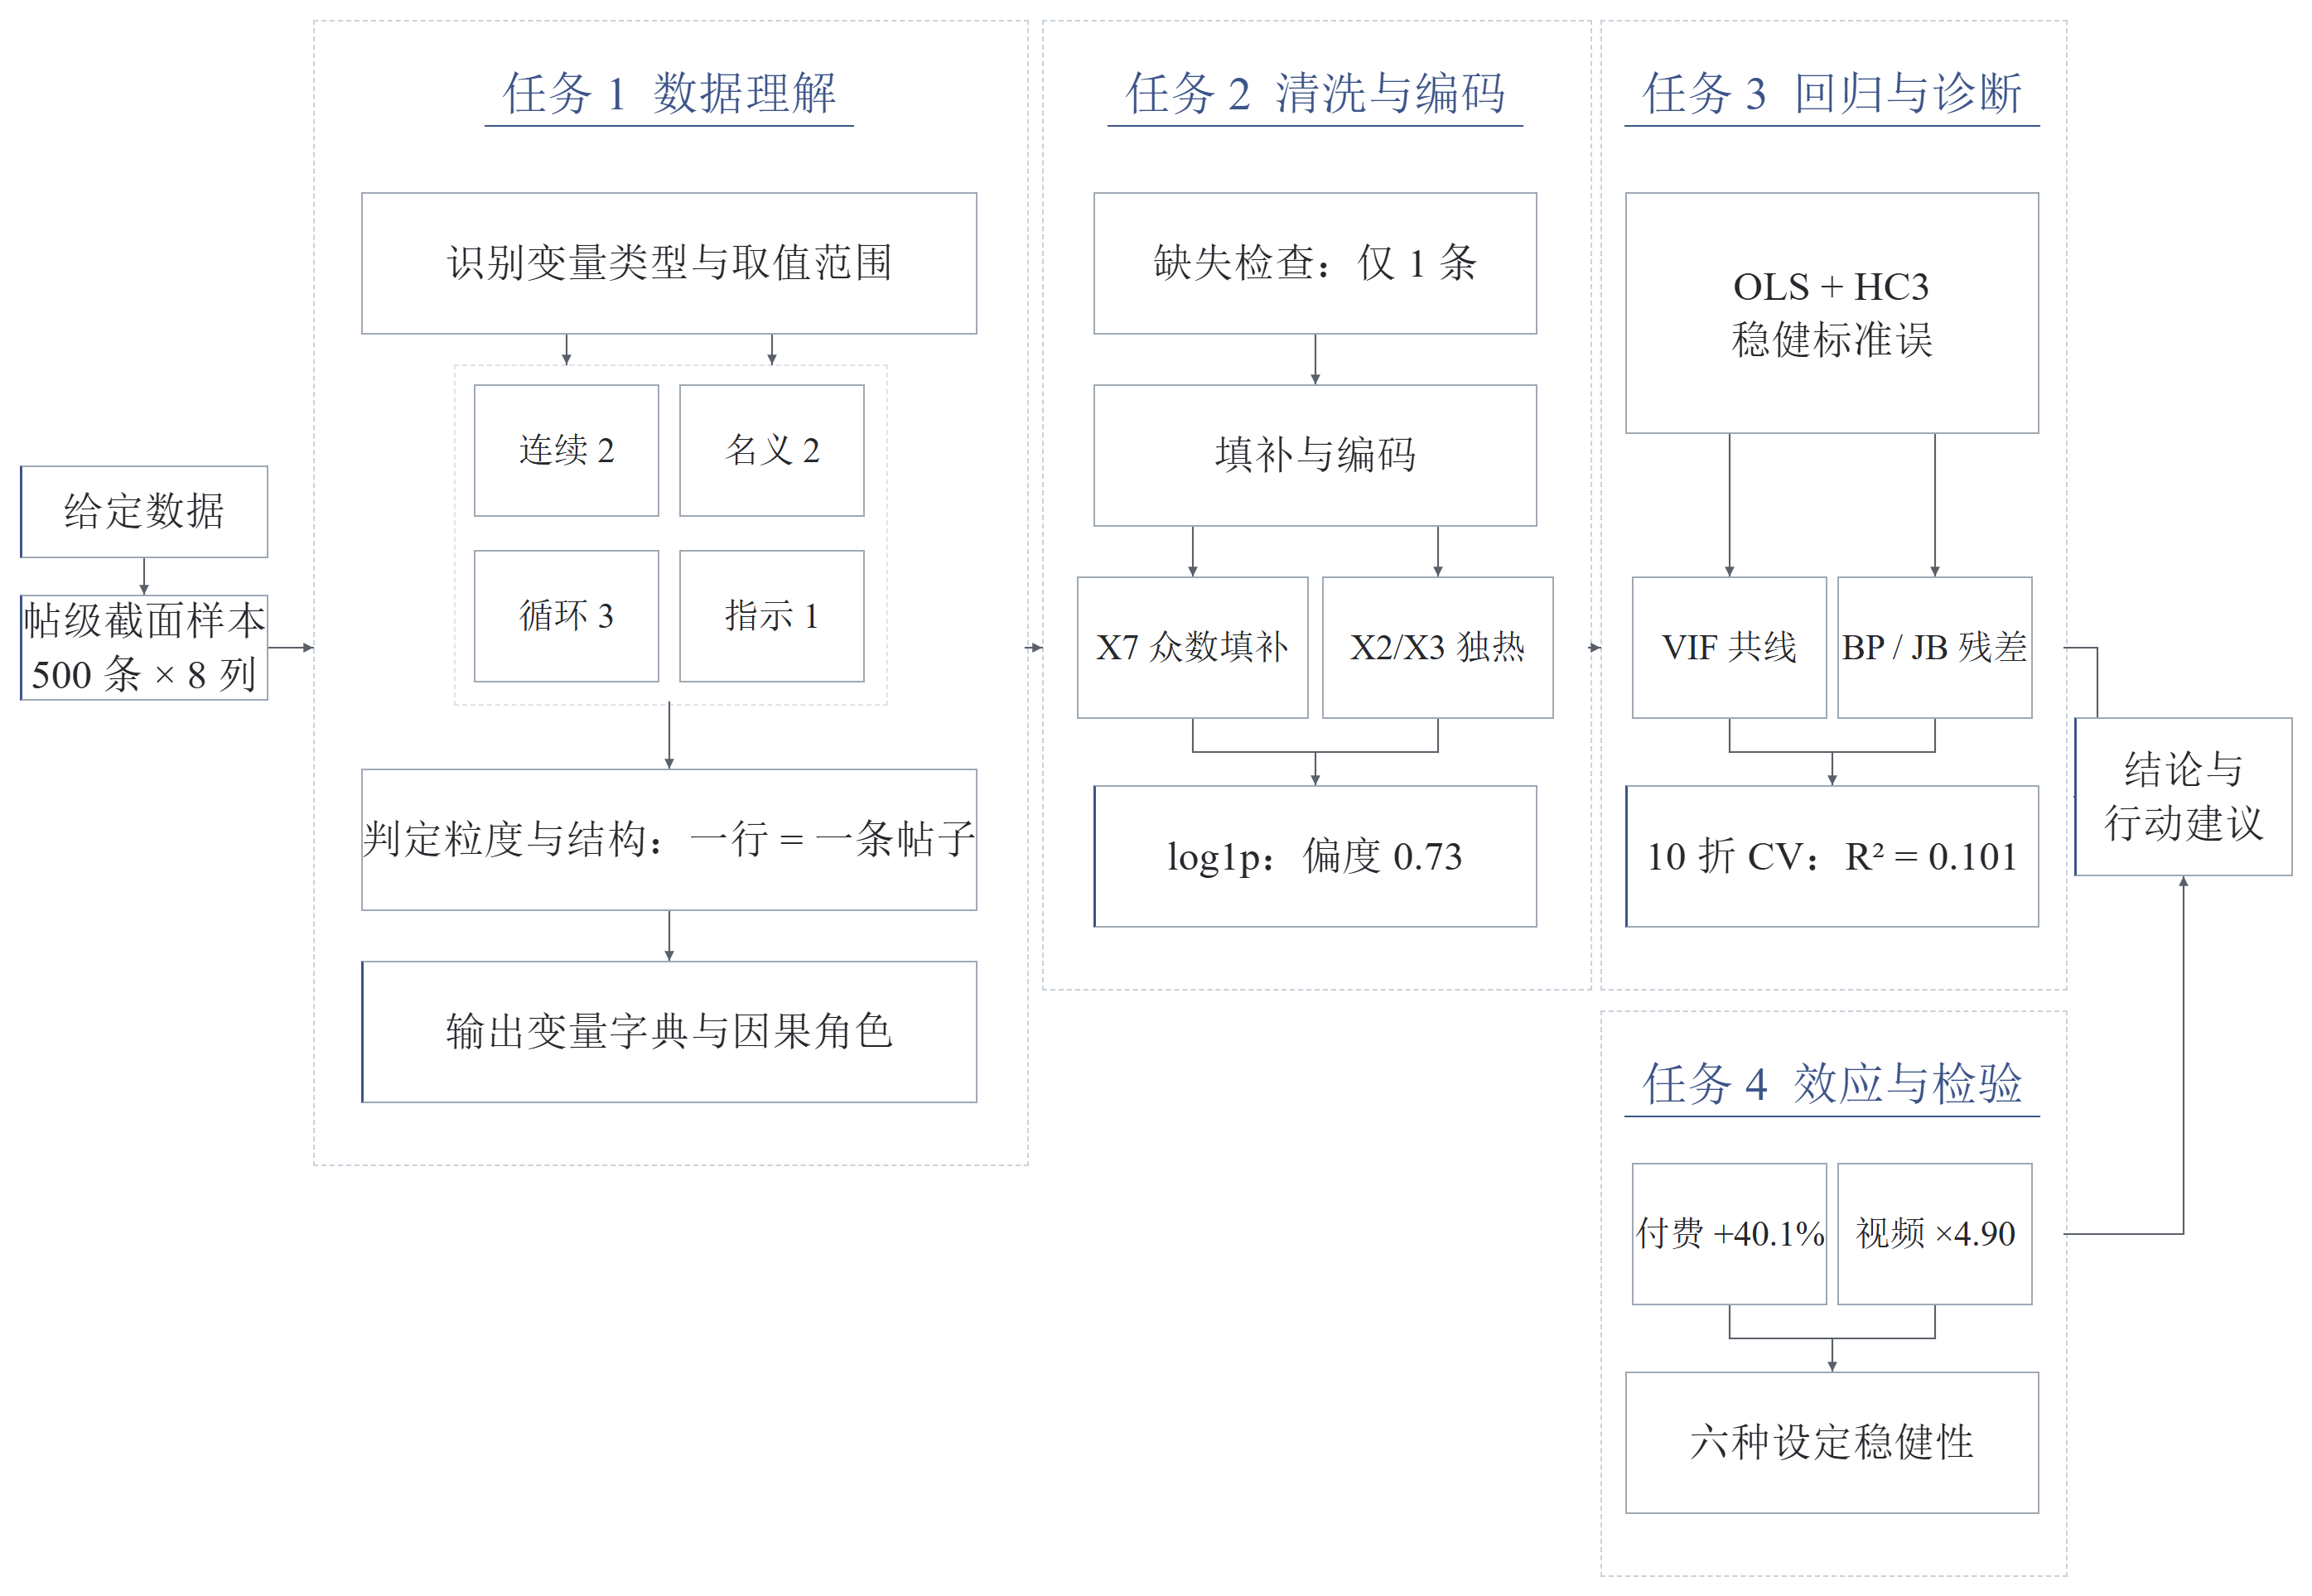
\includegraphics[width=0.90\textwidth]{../求解/临时产物/图0_技术路线.png}
  \caption{技术路线：四环节任务流与关键判据}
  \label{fig:route}
\end{figure}


% ════════════════════════════════════════════
% 基本假设（03.模型假设.tex）
% ════════════════════════════════════════════
\subsection{基本假设}

为明确分析边界，本报告做出以下假设。

\textbf{假设1：} 同一主页的 500 条帖子在给定协变量下相互独立，单条帖子的曝光不显著挤占其他帖子的推荐流量，因而可作为独立样本做统计推断。

\textbf{假设2：} 付费标记的 1 条缺失为完全随机缺失，众数填补不改变参数方向与量级，缺失处理方案的差异可忽略。

\textbf{假设3：} log1p 曝光量的条件均值对解释变量呈可加线性关系，月份固定效应能够吸收粉丝规模随时间累积的趋势。

\textbf{假设4：} 在控制内容类型、主题与发布时机后，付费标记与内容类型同随机扰动不相关，反事实预测用于情景比较而非严格的因果识别。

上述假设不改变数据本身，只界定结论的适用范围。若独立性或完全随机缺失不成立，区间估计会偏窄；若线性设定不成立，系数应理解为局部平均效应而非全局因果效应。报告在相应位置说明了这些限制，并用六种设定与缺失处理对照检验结论对假设的敏感程度。

